\chapter{Hạt đồng nhất, nguyên lý biến phân và năng lượng tương quan}
\label{ch:hatdongnhat}

Chương này trang bị ba công cụ mà mọi phương pháp sau đều dùng: (1) quy tắc phản đối xứng của electron, dẫn tới nguyên lý Pauli và định thức Slater; (2) nguyên lý biến phân, ``la bàn'' cho biết một hàm sóng gần đúng tốt hay dở; (3) khái niệm năng lượng tương quan, thước đo cho phần khó nhất của bài toán.

\section{Electron không có tên}

\begin{eli5}[tiền trong tài khoản]
Bạn có hai tờ 100 nghìn trong tài khoản ngân hàng. Không có ``tờ thứ nhất'' hay ``tờ thứ hai'', chỉ có ``200 nghìn''. Electron cũng vậy: mọi electron giống hệt nhau, \textbf{không thể dán nhãn}. Nếu đổi chỗ hai electron, không thí nghiệm nào phân biệt được trước và sau.

Riêng electron còn có một quy tắc kỳ lạ: khi đổi chỗ hai electron trong công thức, hàm sóng \textbf{đổi dấu} (nhân với $-1$), còn xác suất (bình phương của hàm sóng) thì không đổi.

\emph{Chỗ ví dụ ``gãy'':} tiền không có ``dấu trừ khi đổi chỗ''. Quy tắc đổi dấu của electron không có tương tự nào trong đời thường.
\end{eli5}

\begin{congthuc}[tính phản đối xứng]
Ghép vị trí $\vr$ và spin $\omega$ (``lên'' $\uparrow$ hoặc ``xuống'' $\downarrow$) của electron thành một biến $\vx=(\vr,\omega)$. Hàm sóng của mọi hệ electron phải thỏa
\[
\Psi(\ldots,\vx_i,\ldots,\vx_j,\ldots)=-\,\Psi(\ldots,\vx_j,\ldots,\vx_i,\ldots)\qquad\text{với mọi cặp } i,j.
\]
Hamiltonian đối xứng với mọi phép đổi nhãn, nhưng yêu cầu phản đối xứng \emph{không} suy ra được từ đó. Nó là một tiên đề mới của cơ học lượng tử, đứng ngang hàng về mặt logic với chính phương trình Schrödinger \cite{Griffiths2018}. Những hạt tuân theo quy tắc này gọi là \textbf{fermion} (electron, proton, neutron); hạt có hàm sóng đối xứng (không đổi dấu) gọi là \textbf{boson} (photon, nguyên tử $^4$He).
\end{congthuc}

\section{Spin và nguyên lý loại trừ Pauli}

\begin{eli5}[rạp chiếu phim]
Hình dung các \emph{orbital} (vùng không gian mà electron hay có mặt) như các hàng ghế trong rạp chiếu phim. Mỗi hàng chỉ có đúng hai ghế: một ghế ``spin lên'', một ghế ``spin xuống''. Không bao giờ có hai electron ngồi cùng một ghế: đó là \textbf{nguyên lý loại trừ Pauli} \cite{Pauli1925}. Li có 3 electron. Hai người đầu ngồi kín hàng 1s (một lên, một xuống), người thứ ba buộc phải lên hàng sau, hàng 2s.

\emph{Chỗ ví dụ ``gãy'':} electron không ``ngồi'' ở đâu cả; orbital chỉ là công cụ gần đúng; và ``spin lên/xuống'' không phải electron tự quay như con quay.
\end{eli5}

Nguyên lý Pauli không phải là một quy tắc thêm vào, mà là \emph{hệ quả} của tính phản đối xứng. Để thấy điều đó, ta cần một cách viết hàm sóng tự động phản đối xứng: định thức Slater.

\section{Định thức Slater}

Cách đơn giản nhất để tạo hàm sóng nhiều electron là nhân các hàm một electron: $\Psi=\chi_1(\vx_1)\chi_2(\vx_2)\chi_3(\vx_3)$, gọi là \textbf{tích Hartree} \en{Hartree product}. Mỗi $\chi$ là một \textbf{spin-orbital}: tích của một orbital không gian $\varphi(\vr)$ và một hàm spin $\alpha$ ($\uparrow$) hoặc $\beta$ ($\downarrow$). Nhưng tích Hartree ``dán nhãn'' electron (electron 1 ở $\chi_1$\ldots) và không đổi dấu khi đổi chỗ, nên vi phạm tiên đề trên. Slater (1929) nhận ra rằng \textbf{định thức} của ma trận có tính chất đúng như ta cần \cite{Slater1929}: đổi hai hàng thì định thức đổi dấu.

\begin{congthuc}[định thức Slater cho Li]
Đặt $a=\varphi_{1s}\alpha$ (1s, spin lên), $b=\varphi_{1s}\beta$ (1s, spin xuống), $c=\varphi_{2s}\alpha$ (2s, spin lên). Hàng $i$ ứng với electron $i$, cột ứng với spin-orbital:
\[
\Psi_{\rm Li}(\vx_1,\vx_2,\vx_3)=\frac{1}{\sqrt{3!}}
\begin{vmatrix}
a(\vx_1) & b(\vx_1) & c(\vx_1)\\
a(\vx_2) & b(\vx_2) & c(\vx_2)\\
a(\vx_3) & b(\vx_3) & c(\vx_3)
\end{vmatrix}
\]
Khai triển ra đủ $3!=6$ số hạng:
\[
\Psi_{\rm Li}=\tfrac{1}{\sqrt6}\big[a_1b_2c_3-a_1c_2b_3-b_1a_2c_3+b_1c_2a_3+c_1a_2b_3-c_1b_2a_3\big],
\]
với $a_1$ là viết tắt của $a(\vx_1)$. Hệ số $1/\sqrt{6}$ để hàm sóng chuẩn hóa.

Ba tính chất của định thức cho ra ba định luật vật lý:
\begin{itemize}
\item \textbf{Đổi hai hàng} (đổi chỗ hai electron) thì định thức đổi dấu: đúng tiên đề phản đối xứng.
\item \textbf{Hai cột giống nhau} (hai electron cùng spin-orbital) thì định thức bằng 0: đó chính là \textbf{nguyên lý Pauli}. Thử nhét cả ba electron vào 1s: $a, b, a$ có cột 1 và 3 trùng nhau, nên $\Psi\equiv0$. Cấu hình 1s$^3$ không tồn tại.
\item \textbf{Hai hàng giống nhau} (hai electron cùng spin ở cùng một điểm) thì định thức bằng 0: hai electron cùng spin không bao giờ gặp nhau. Quanh mỗi electron có một ``vùng cấm'' với các electron cùng spin, gọi là \textbf{lỗ Fermi} \en{Fermi hole}.
\end{itemize}
\end{congthuc}

\begin{hieulam}[``electron số 3 là electron 2s'']
Trong định thức Slater, \emph{mọi} electron xuất hiện trong \emph{mọi} spin-orbital (nhìn 6 số hạng ở trên: electron 1 có lúc ở $a$, lúc ở $b$, lúc ở $c$). Câu ``Li có hai electron 1s và một electron 2s'' chỉ là cách nói tắt cho ``định thức được dựng từ các spin-orbital 1s$\uparrow$, 1s$\downarrow$, 2s$\uparrow$''.
\end{hieulam}

\begin{hieulam}[``nguyên lý Pauli là một lực đẩy'']
Không có lực nào cả. Electron cùng spin ``tránh nhau'' vì một ràng buộc thuần túy hình học của tính phản đối xứng. Griffiths viết về ``lực trao đổi'': \emph{``it's not really a force at all --- no physical agency is pushing on the particles; rather, it is a purely geometrical consequence of the symmetrization requirement''} \cite{Griffiths2018}.
\end{hieulam}

\subsection{Vì sao electron thứ ba vào 2s mà không vào 2p?}
Pauli chỉ nói 1s đã đầy. Còn việc chọn 2s thay vì 2p là hiệu ứng của lực đẩy giữa các electron. Trong hydro, 2s và 2p có cùng năng lượng. Trong Li, 2p cao hơn 2s tới $1.848\eV$; đó chính là vạch đỏ 671\,nm làm ngọn lửa muối liti có màu đỏ son \cite{NIST-ASD}. Nguyên nhân là orbital 2s có một phần nhỏ ``xuyên'' vào sát hạt nhân, bên trong lớp 1s, nên bị hai electron 1s \textbf{che chắn} \en{screening} ít hơn. Electron 2p gần như chỉ ``thấy'' điện tích $+1$ (hạt nhân $+3$ bị hai electron 1s che mất $-2$), còn electron 2s thấy khoảng $+1.26$.

Hình~\ref{fig:matdo} (tính bằng code của chương~\ref{ch:hf}) cho thấy rõ cấu trúc lớp vỏ: hai electron 1s tập trung rất gần hạt nhân (đỉnh ở $r\approx0.36\bohr$), electron 2s nằm xa hơn gần 9 lần (đỉnh ở $r\approx3.1\bohr$), nhưng vẫn có một ``thùy'' nhỏ bên trong lớp 1s, ngăn cách bởi một \textbf{nút} \en{node} tại $r\approx0.83\bohr$.

\begin{figure}[h]
\centering
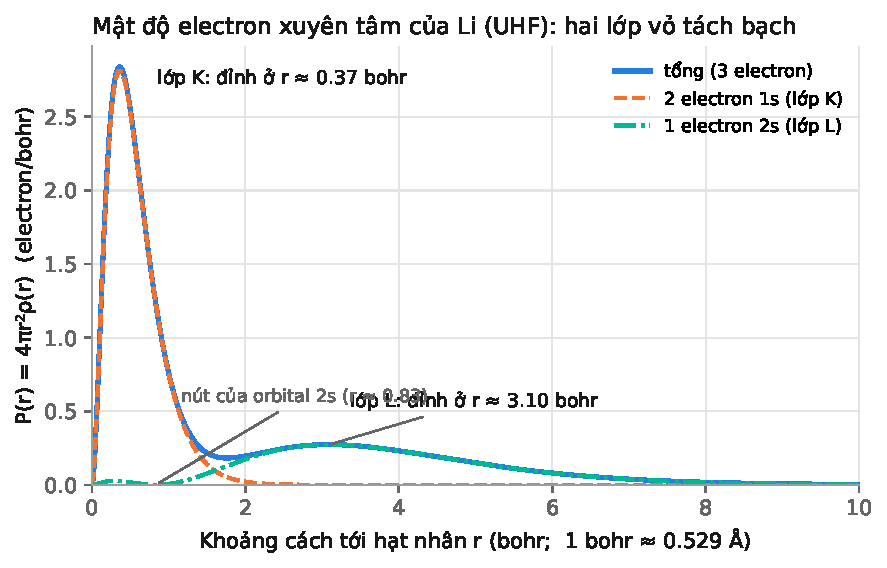
\includegraphics[width=0.8\textwidth]{02_mat_do_xuyen_tam.pdf}
\caption{Mật độ electron xuyên tâm $P(r)=4\pi r^2\rho(r)$ của Li (Hartree--Fock không hạn chế, tập cơ sở aug-cc-pCVQZ). Diện tích dưới đường tổng bằng đúng 3 electron. Thùy nhỏ của 2s bên trong lớp 1s là phần ``xuyên thấu'' giúp 2s có năng lượng thấp hơn 2p. (Script \code{02\_hartree\_fock.py})}
\label{fig:matdo}
\end{figure}

\subsection{Spin toàn phần: Li là một ``doublet''}
Hai electron 1s có spin ngược nhau nên tổng spin của cặp bằng 0. Electron 2s không có cặp, nên spin toàn phần của Li là $S=\tfrac12$ và có $2S+1=2$ cách định hướng: trạng thái \textbf{doublet}, ký hiệu $1s^22s\;{}^2S_{1/2}$. Vì có một electron lẻ, Li thuộc loại hệ \textbf{vỏ mở} \en{open-shell}. Chương~\ref{ch:hf} sẽ cho thấy điều này đòi hỏi hai biến thể của phương pháp Hartree--Fock (ROHF và UHF).

\section{Nguyên lý biến phân}\label{sec:bienphan}

\begin{eli5}[tìm đáy thung lũng trong sương mù]
Bạn phải tìm điểm thấp nhất của một thung lũng chìm trong sương mù. Bạn không nhìn thấy đáy, nhưng biết chắc một điều: \emph{mọi chỗ bạn đứng đều cao hơn hoặc bằng đáy}. Đi thử nhiều chỗ, chỗ thấp nhất bạn tìm được luôn là một ``cận trên'' của độ sâu thật. Đi càng khéo, càng gần đáy.

Trong lượng tử, ``chỗ đứng'' là một hàm sóng đoán thử, còn ``độ cao'' là năng lượng tính từ hàm đó. Năng lượng của hàm đoán thử không bao giờ thấp hơn năng lượng cơ bản thật.

\emph{Chỗ ví dụ ``gãy'':} ``thung lũng'' ở đây nằm trong một không gian vô hạn chiều (không gian các hàm), và bạn phải đi đúng ``lối'' (hàm phản đối xứng). Đi sai lối có thể rơi xuống một thung lũng ``cấm'' sâu hơn đáy thật, như sẽ thấy ở hình~\ref{fig:bacthang}.
\end{eli5}

\begin{congthuc}[định lý biến phân]
Với mọi hàm thử $\Phi$ có đúng tính đối xứng (phản đối xứng với electron),
\[
E[\Phi]=\frac{\langle\Phi|\Hhat|\Phi\rangle}{\langle\Phi|\Phi\rangle}\;\ge\;E_0 ,
\]
dấu bằng xảy ra khi và chỉ khi $\Phi$ là hàm sóng cơ bản. Ở đây $\langle\Phi|\Hhat|\Phi\rangle=\int\Phi^*\,\Hhat\,\Phi\,d\tau$ là tích phân trên mọi tọa độ và spin.

\textbf{Chứng minh (3 dòng).} Khai triển $\Phi=\sum_n c_n\Psi_n$ theo các trạng thái riêng chính xác $\Hhat\Psi_n=E_n\Psi_n$ (chúng tạo thành một cơ sở trực chuẩn). Khi đó
\[
E[\Phi]=\frac{\sum_n|c_n|^2E_n}{\sum_n|c_n|^2}\;\ge\;\frac{\sum_n|c_n|^2E_0}{\sum_n|c_n|^2}=E_0 ,
\]
vì mọi $E_n\ge E_0$. Năng lượng của hàm thử là một trung bình có trọng số của các $E_n$, và trung bình không thể nhỏ hơn số nhỏ nhất.

\textbf{Một hệ quả dễ chịu.} Nếu hàm thử sai lệch cỡ $\epsilon$ so với hàm đúng, năng lượng chỉ sai lệch cỡ $\epsilon^2$. Hàm sóng sai 10\% thì năng lượng chỉ sai cỡ 1\%. Vì thế năng lượng thường tốt hơn nhiều so với hàm sóng tạo ra nó. Ngược lại, năng lượng tốt chưa chắc các tính chất khác (như mật độ ở sát hạt nhân) cũng tốt.
\end{congthuc}

Gần như mọi phương pháp trong tài liệu này dựa trên nguyên lý biến phân: Hartree--Fock, CI, Monte Carlo biến phân, mạng nơ-ron. Hai ngoại lệ quan trọng là MP2 và Coupled Cluster (chương~\ref{ch:sauhf}): chúng \emph{không} cho cận trên.

\subsection{Ví dụ khởi động: nguyên tử heli}
Thử hàm $\Phi=e^{-\zeta(r_1+r_2)}$: cả hai electron ở orbital kiểu 1s, nhưng thay điện tích hạt nhân thật $Z=2$ bằng một ``điện tích hiệu dụng'' $\zeta$ có thể điều chỉnh. (Với hai electron spin ngược nhau, phần không gian đối xứng; tính phản đối xứng nằm trong phần spin.) Tính các tích phân (xem \cite{Griffiths2018}, chương 8) cho:
\[
E(\zeta)=\underbrace{\zeta^2}_{\text{động năng}}\;\underbrace{-\,2Z\zeta}_{\text{hút hạt nhân}}\;+\;\underbrace{\tfrac58\zeta}_{\text{đẩy nhau}} .
\]
Đạo hàm bằng 0 cho $\zeta^*=Z-\tfrac{5}{16}=\tfrac{27}{16}=1.6875$ và $E(\zeta^*)=-(27/16)^2=-2.8477\Ha$, cao hơn giá trị chính xác $-2.9037\Ha$ đúng như định lý khẳng định (hình~\ref{fig:he}). Ý nghĩa vật lý: $\zeta^*<Z$, vì mỗi electron bị electron kia \textbf{che chắn} một phần điện tích hạt nhân.

\begin{figure}[h]
\centering
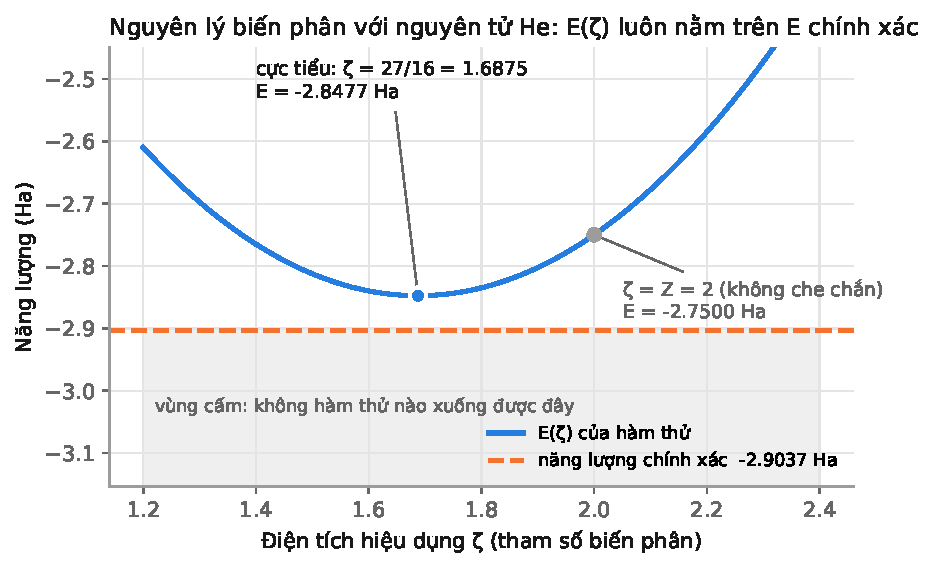
\includegraphics[width=0.78\textwidth]{01_bien_phan_he.pdf}
\caption{Nguyên lý biến phân với nguyên tử He. Mọi giá trị của tham số $\zeta$ cho năng lượng cao hơn đáp án chính xác (vạch cam). Giá trị tốt nhất $\zeta^*=27/16$ vẫn sai $56\mHa$. (Script \code{01\_nen\_tang.py})}
\label{fig:he}
\end{figure}

\subsection{Áp dụng cho Li: bậc thang năng lượng}
Với Li, dùng định thức $|1s\!\uparrow 1s\!\downarrow 2s\!\uparrow|$ với các orbital kiểu hydro có chung điện tích hiệu dụng $\zeta$. Tính các tích phân theo quy tắc Slater--Condon \cite{Szabo1996} được
\[
E(\zeta)=\tfrac98\zeta^2-\tfrac{27}{4}\zeta+\Big(\underbrace{\tfrac58}_{J_{1s1s}}+\underbrace{\tfrac{34}{81}}_{2J_{1s2s}}-\underbrace{\tfrac{16}{729}}_{K_{1s2s}}\Big)\zeta ,
\]
cực tiểu tại $\zeta^*=2.5454$ với $E=-7.2891\Ha$. Số hạng $K_{1s2s}$ mang dấu trừ là \textbf{năng lượng trao đổi} \en{exchange energy}: nó chỉ xuất hiện giữa hai electron \emph{cùng spin} (1s$\uparrow$ và 2s$\uparrow$) và là ``dấu vết'' năng lượng của lỗ Fermi. Chương~\ref{ch:hf} sẽ nói kỹ về $J$ và $K$.

\begin{figure}[h]
\centering
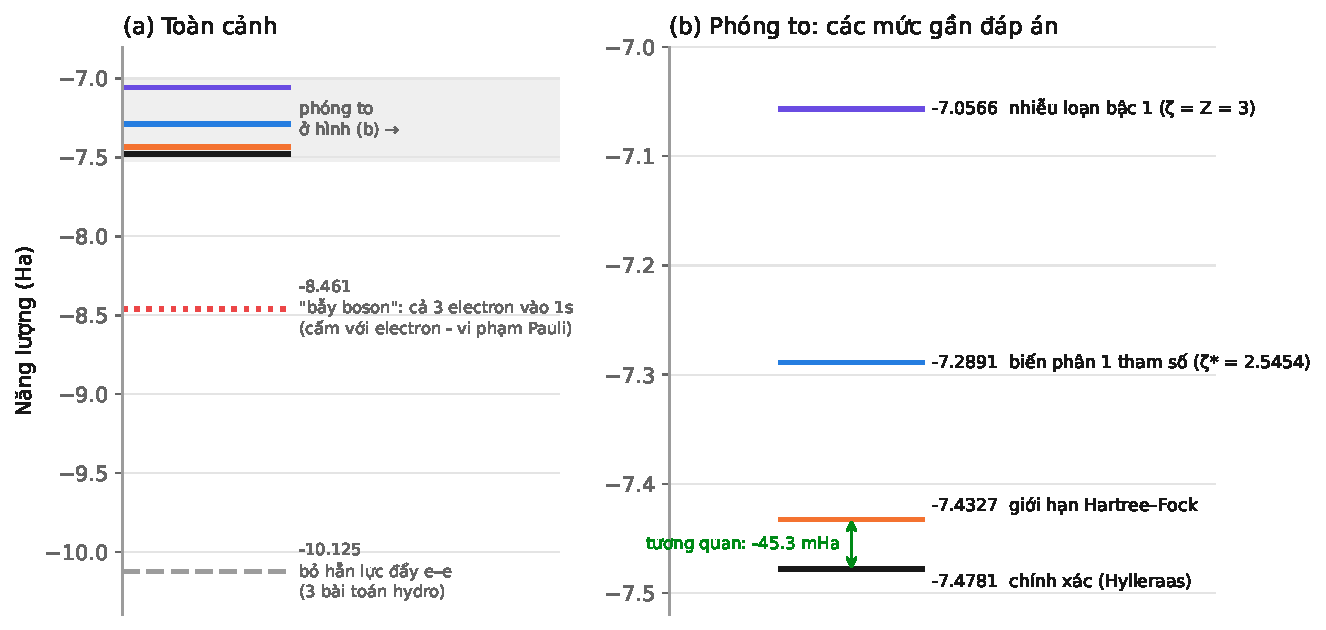
\includegraphics[width=\textwidth]{01_bac_thang_li.pdf}
\caption{Các mức xấp xỉ năng lượng của Li. Bỏ lực đẩy cho $-10.125\Ha$ (không phải biến phân vì đã đổi Hamiltonian). Hàm một tham số cho $-7.289\Ha$, giới hạn Hartree--Fock là $-7.433\Ha$, đáp án là $-7.478\Ha$. Vạch đỏ chấm là ``bẫy boson'': nếu quên tính phản đối xứng và cho cả 3 electron vào 1s, năng lượng xuống tới $-8.461\Ha$, \emph{thấp hơn} đáp án thật. (Script \code{01\_nen\_tang.py})}
\label{fig:bacthang}
\end{figure}

\begin{hieulam}[cái bẫy boson]
Hàm thử cho cả 3 electron vào 1s cho $E=-8.461\Ha$, thấp hơn năng lượng thật của Li. Có mâu thuẫn với nguyên lý biến phân không? Không: nguyên lý chỉ đảm bảo cận trên cho trạng thái thấp nhất \emph{trong lớp đối xứng mà hàm thử thuộc về}. Hàm không phản đối xứng thuộc ``thế giới boson'', nơi trạng thái thấp nhất nằm dưới trạng thái thấp nhất của fermion. Bài học: hàm thử \emph{bắt buộc} phải đúng đối xứng.
\end{hieulam}

\section{Năng lượng tương quan}\label{sec:tuongquan}

\begin{eli5}[quảng trường đông người]
Phương pháp Hartree--Fock (chương~\ref{ch:hf}) là hàm sóng dạng \emph{một} định thức Slater tốt nhất có thể. Nó giống như mỗi người trong một quảng trường đông đúc chỉ phản ứng với ``độ đông trung bình'' của đám đông, không nhìn từng người cụ thể. Ngoài đời, mọi người \emph{né nhau} từng bước một. Phần năng lượng mà cách nhìn ``trung bình'' bỏ sót gọi là \textbf{năng lượng tương quan}.

Quanh mỗi electron có hai ``bong bóng riêng tư''. \textbf{Lỗ Fermi} đẩy các electron \emph{cùng spin} ra xa; nó do Pauli gây ra và Hartree--Fock đã mô tả đúng. \textbf{Lỗ Coulomb} là phần né nhau thêm do lực đẩy tĩnh điện, nhất là giữa các electron \emph{ngược spin}; Hartree--Fock bỏ sót phần này.
\end{eli5}

\begin{congthuc}[định nghĩa của Löwdin]
\[
\Ecorr = E_{\text{chính xác}} - \EHF \;<\; 0 .
\]
$\EHF$ là năng lượng Hartree--Fock ở giới hạn tập cơ sở vô hạn. $\Ecorr$ luôn âm vì Hartree--Fock là phương pháp biến phân \cite{Lowdin1955}. Với Li:
\[
\Ecorr(\text{Li})=-7.478\,060-(-7.432\,727)=-0.045\,333\Ha=-1.234\eV .
\]
\end{congthuc}

Năng lượng tương quan chỉ chiếm 0.6\% tổng năng lượng của Li. Có nên bỏ qua không? Không, vì nó cỡ $28$\,kcal/mol, gấp 28 lần ``độ chính xác hóa học'' $1$\,kcal/mol ($1.6\mHa$). Đó là mức chính xác cần để dự đoán đúng một phản ứng hóa học có xảy ra hay không. Năng lượng liên kết hóa học cũng chỉ cỡ vài eV. Tính sai $\Ecorr$ là tính sai hóa học.

\begin{table}[h]
\centering\small
\caption{Năng lượng tương quan của vài nguyên tử và ion nhẹ \cite{King2018,KogaThakkar1996,Wang2012,Hornyak2019}.}
\label{tab:ecorr}
\begin{tabular}{@{}lrrrr@{}}
\toprule
Hệ & $\Ecorr$ (Ha) & $\Ecorr$ (eV) & kcal/mol & \% của $|E|$ \\
\midrule
He & $-0.042\,044$ & $-1.144$ & $-26.4$ & 1.45 \\
Li$^+$ (1s$^2$) & $-0.043\,498$ & $-1.184$ & $-27.3$ & 0.60 \\
Li (1s$^2$2s) & $-0.045\,333$ & $-1.234$ & $-28.4$ & 0.61 \\
Be (1s$^2$2s$^2$) & $-0.094\,333$ & $-2.567$ & $-59.2$ & 0.64 \\
\bottomrule
\end{tabular}
\end{table}

Một nhận xét thú vị từ bảng~\ref{tab:ecorr}: $\Ecorr(\text{Li}^+)$ đã bằng khoảng 96\% $\Ecorr(\text{Li})$. Tức là phần lớn tương quan của Li nằm ở \textbf{cặp electron lõi 1s$^2$}, hai electron ngược spin bị nén sát nhau quanh hạt nhân. Electron 2s ở xa nên chỉ đóng góp thêm khoảng $-1.8\mHa$. Chương~\ref{ch:sauhf} sẽ cho thấy hệ quả thực tế: tập cơ sở phải có đủ hàm để mô tả tương quan ở lõi.

\subsection{Tương quan động và tương quan tĩnh}
Người ta chia tương quan làm hai loại \cite{HollettGill2011}. \textbf{Tương quan động} \en{dynamic correlation} là việc electron né nhau ở khoảng cách ngắn, khắp mọi nơi và mọi lúc. \textbf{Tương quan tĩnh} \en{static correlation} xuất hiện khi có vài cấu hình electron gần như cùng năng lượng, nên một định thức duy nhất là không đủ. Be là ví dụ kinh điển: cấu hình 1s$^2$2p$^2$ trộn mạnh với 1s$^2$2s$^2$. Li chỉ có một electron hóa trị nên tương quan gần như hoàn toàn là \emph{động}. Đó là một lý do Li là ví dụ ``sạch'' để học.

\subsection{Điều kiện ``mũi nhọn'' của Kato}\label{sec:cusp}
Khi hai hạt tích điện tiến sát nhau ($r\to0$), thế Coulomb $\pm1/r$ tiến ra vô cùng. Để tổng $\Hhat\Psi$ vẫn hữu hạn, động năng phải ``bù'' lại vô cùng đó, và điều này buộc hàm sóng có một điểm gãy nhọn như đỉnh lều. Kato chứng minh điều này năm 1957 \cite{Kato1957}:

\begin{congthuc}[điều kiện cusp]
\begin{itemize}
\item Electron--hạt nhân: $\dfrac{\partial\bar\Psi}{\partial r_i}\Big|_{r_i=0}=-Z\,\Psi\big|_{r_i=0}$. Với hydro $\psi=e^{-Zr}$, ta có đúng $\psi'(0)=-Z\psi(0)$.
\item Hai electron ngược spin: $\dfrac{\partial\bar\Psi}{\partial r_{ij}}\Big|_{r_{ij}=0}=+\tfrac12\,\Psi\big|_{r_{ij}=0}$, tức gần điểm va chạm $\Psi\approx\Psi(0)(1+\tfrac12r_{ij})$.
\item Hai electron cùng spin: $\Psi=0$ tại điểm va chạm (lỗ Fermi), và hệ số tương ứng là $\tfrac14$.
\end{itemize}
($\bar\Psi$ là trung bình trên mặt cầu nhỏ quanh điểm va chạm.)
\end{congthuc}

Điều kiện cusp electron--electron giải thích vì sao các phương pháp dựng hàm sóng từ orbital (CI, Coupled Cluster) hội tụ \emph{chậm}: tổ hợp của các hàm mượt rất khó tạo ra một điểm gãy nhọn theo $r_{12}$. Với He, dù dùng orbital tới mômen động lượng $l=15$, CI vẫn sai $4.3$\,µHa \cite{Ruiz2021}. Lời giải, từ Hylleraas năm 1929, là đưa thẳng $r_{12}$ vào hàm sóng. Đó là bí quyết của các con số 15 chữ số ở bảng~\ref{tab:chuso}, và cũng là ý tưởng của thừa số Jastrow trong Monte Carlo lượng tử (chương~\ref{ch:qmc}).

\section{Bảng giá trị tham chiếu cho Li}

\begin{table}[h]
\centering\small
\caption{Các giá trị tham chiếu dùng xuyên suốt tài liệu (phi tương đối tính, hạt nhân cố định, trừ năng lượng ion hóa thực nghiệm).}
\label{tab:thamchieu}
\begin{tabularx}{\textwidth}{@{}Xrl@{}}
\toprule
Đại lượng & Giá trị & Nguồn \\
\midrule
Năng lượng chính xác $E(\text{Li})$ & $-7.478\,060\,323\,910\Ha$ & \cite{Wang2012,PKP2009} \\
Giới hạn Hartree--Fock $\EHF(\text{Li})$ (ROHF) & $-7.432\,726\,931\Ha$ & \cite{KogaThakkar1996} \\
Năng lượng tương quan $\Ecorr(\text{Li})$ & $-0.045\,333\Ha$ & tính từ hai dòng trên \\
$E(\text{Li}^+)$, cấu hình 1s$^2$ & $-7.279\,913\,412\,669\Ha$ & \cite{Nakashima2007} \\
$E(\text{Li}^{2+})$, cấu hình 1s & $-4.5\Ha$ (chính xác) & lời giải hydro \\
Năng lượng ion hóa thứ nhất, thực nghiệm & $5.391\,715\eV$ & \cite{NIST-ASD} \\
Năng lượng ion hóa thứ nhất, từ $E(\text{Li}^+)-E(\text{Li})$ & $5.391\,85\eV$ & tính toán \\
\bottomrule
\end{tabularx}
\end{table}

\begin{ghinho}
\begin{itemize}
\item Electron là fermion: hàm sóng đổi dấu khi đổi chỗ hai electron. Định thức Slater tự động thỏa điều này, và nguyên lý Pauli là hệ quả trực tiếp.
\item Nguyên lý biến phân: năng lượng của mọi hàm thử (đúng đối xứng) đều $\ge E_0$. Sai số năng lượng là bậc hai theo sai số hàm sóng.
\item Năng lượng tương quan $\Ecorr=E_{\text{chính xác}}-\EHF$. Với Li là $-45.3\mHa$, chỉ 0.6\% tổng năng lượng nhưng gấp 28 lần độ chính xác hóa học. Phần lớn nằm ở cặp lõi 1s$^2$.
\item Hàm sóng chính xác có ``mũi nhọn'' (cusp) khi hai hạt va chạm. Hàm dựng từ orbital mượt khó tạo ra mũi nhọn này, nên hội tụ chậm.
\end{itemize}
\end{ghinho}
